%\documentclass{article}
\documentclass[oneside]{report} 

\usepackage[UTF8, fntef]{ctex}
\usepackage{graphicx}
\usepackage{epstopdf}

%\usepackage[a4paper, total={6in, 10in}]{geometry}
\usepackage[left=2cm,right=4.cm,top=2cm,bottom=2cm]{geometry} 
%\usepackage{setspace}
%\singlespacing
%\onehalfspacing
%\doublespacing

\usepackage[backref]{hyperref} 
\usepackage{amsmath}
\usepackage{booktabs} % 导入三线表需要的宏包
\usepackage{caption}
\usepackage{float} 
%
\usepackage{subfigure}
%\usepackage{subcaption}
\usepackage[numbers,sort&compress]{natbib}%参考文献顺序
\usepackage{siunitx}%\SI{}{\degreeCelsius}
\hypersetup{hidelinks}



%----------------------------------------------
%----------------------------------------------
%
\usepackage{amssymb}
\usepackage{amsfonts}


\usepackage{color, xcolor}
\usepackage{soul}


\usepackage{hyperref}
%
\hypersetup{
    colorlinks=true,
    linkcolor=black, %blue,
    filecolor=black, %magenta,      
    urlcolor=black, %blue, %cyan,
    pdftitle={Sharelatex Example},
    bookmarks=true,
    pdfpagemode=FullScreen,
    linktoc=all  %set to all if you want both sections and subsections linked
}


% todonotes
\usepackage[colorinlistoftodos,
%textsize=scriptsize,
bordercolor=white
%, textcolor=orange!80!black!100
, color=lime!33
]{todonotes}
\setlength{\marginparwidth}{3.4cm}
\newcommand{\donein}{\todo[color=blue!11,inline]}
\newcommand{\done}{\todo[color=blue!11]}

%----------------------------------------------
%----------------------------------------------



\begin{document}


\chapter*{学习报告20230925}

\section*{文献研读}
近两周,我阅读了7篇中文综述,对化学蓄热(CHS)的研究现状、技术路线及其特性、研究热点有了总体上的了解。

如图\ref{fig:研究角度},目前CHS所使用的反应类型按反应体系状态分为化学吸附、化学吸收、物理吸收、物理吸附、纯化学(气-气)五种,其中最受关注的是化学吸附。化学吸附有更高的储能密度,反应器结构较为简单,一定程度上减少了腐蚀和漏液。其中,关于水合盐的研究最多,已经证明与多孔载体的复合材料可以提高水合盐的储热性能、优化其温度范围。目前在该方面的研究方法集中在选择比较不同物质,以及通过复合材料调控其物性。

除了在材料的角度,另一个关注点是反应器装置。宏观上,将反应装置氛围开式、闭式,分别适用于不同特点的反应类型,并各具优缺点。从微观上分析双级孔隙度模型传热传质的性能,使用反应动力学方程、连续方程、能量方程建立数学模型,以对吸收床传热传质性能进行优化。对文献中提到的各种材料和装置进行整理和对比,可以从图\ref{fig:材料对比}中看出各种材料所属类别、适用装置以及储热性能。


\begin{figure}[H]
    \centering
    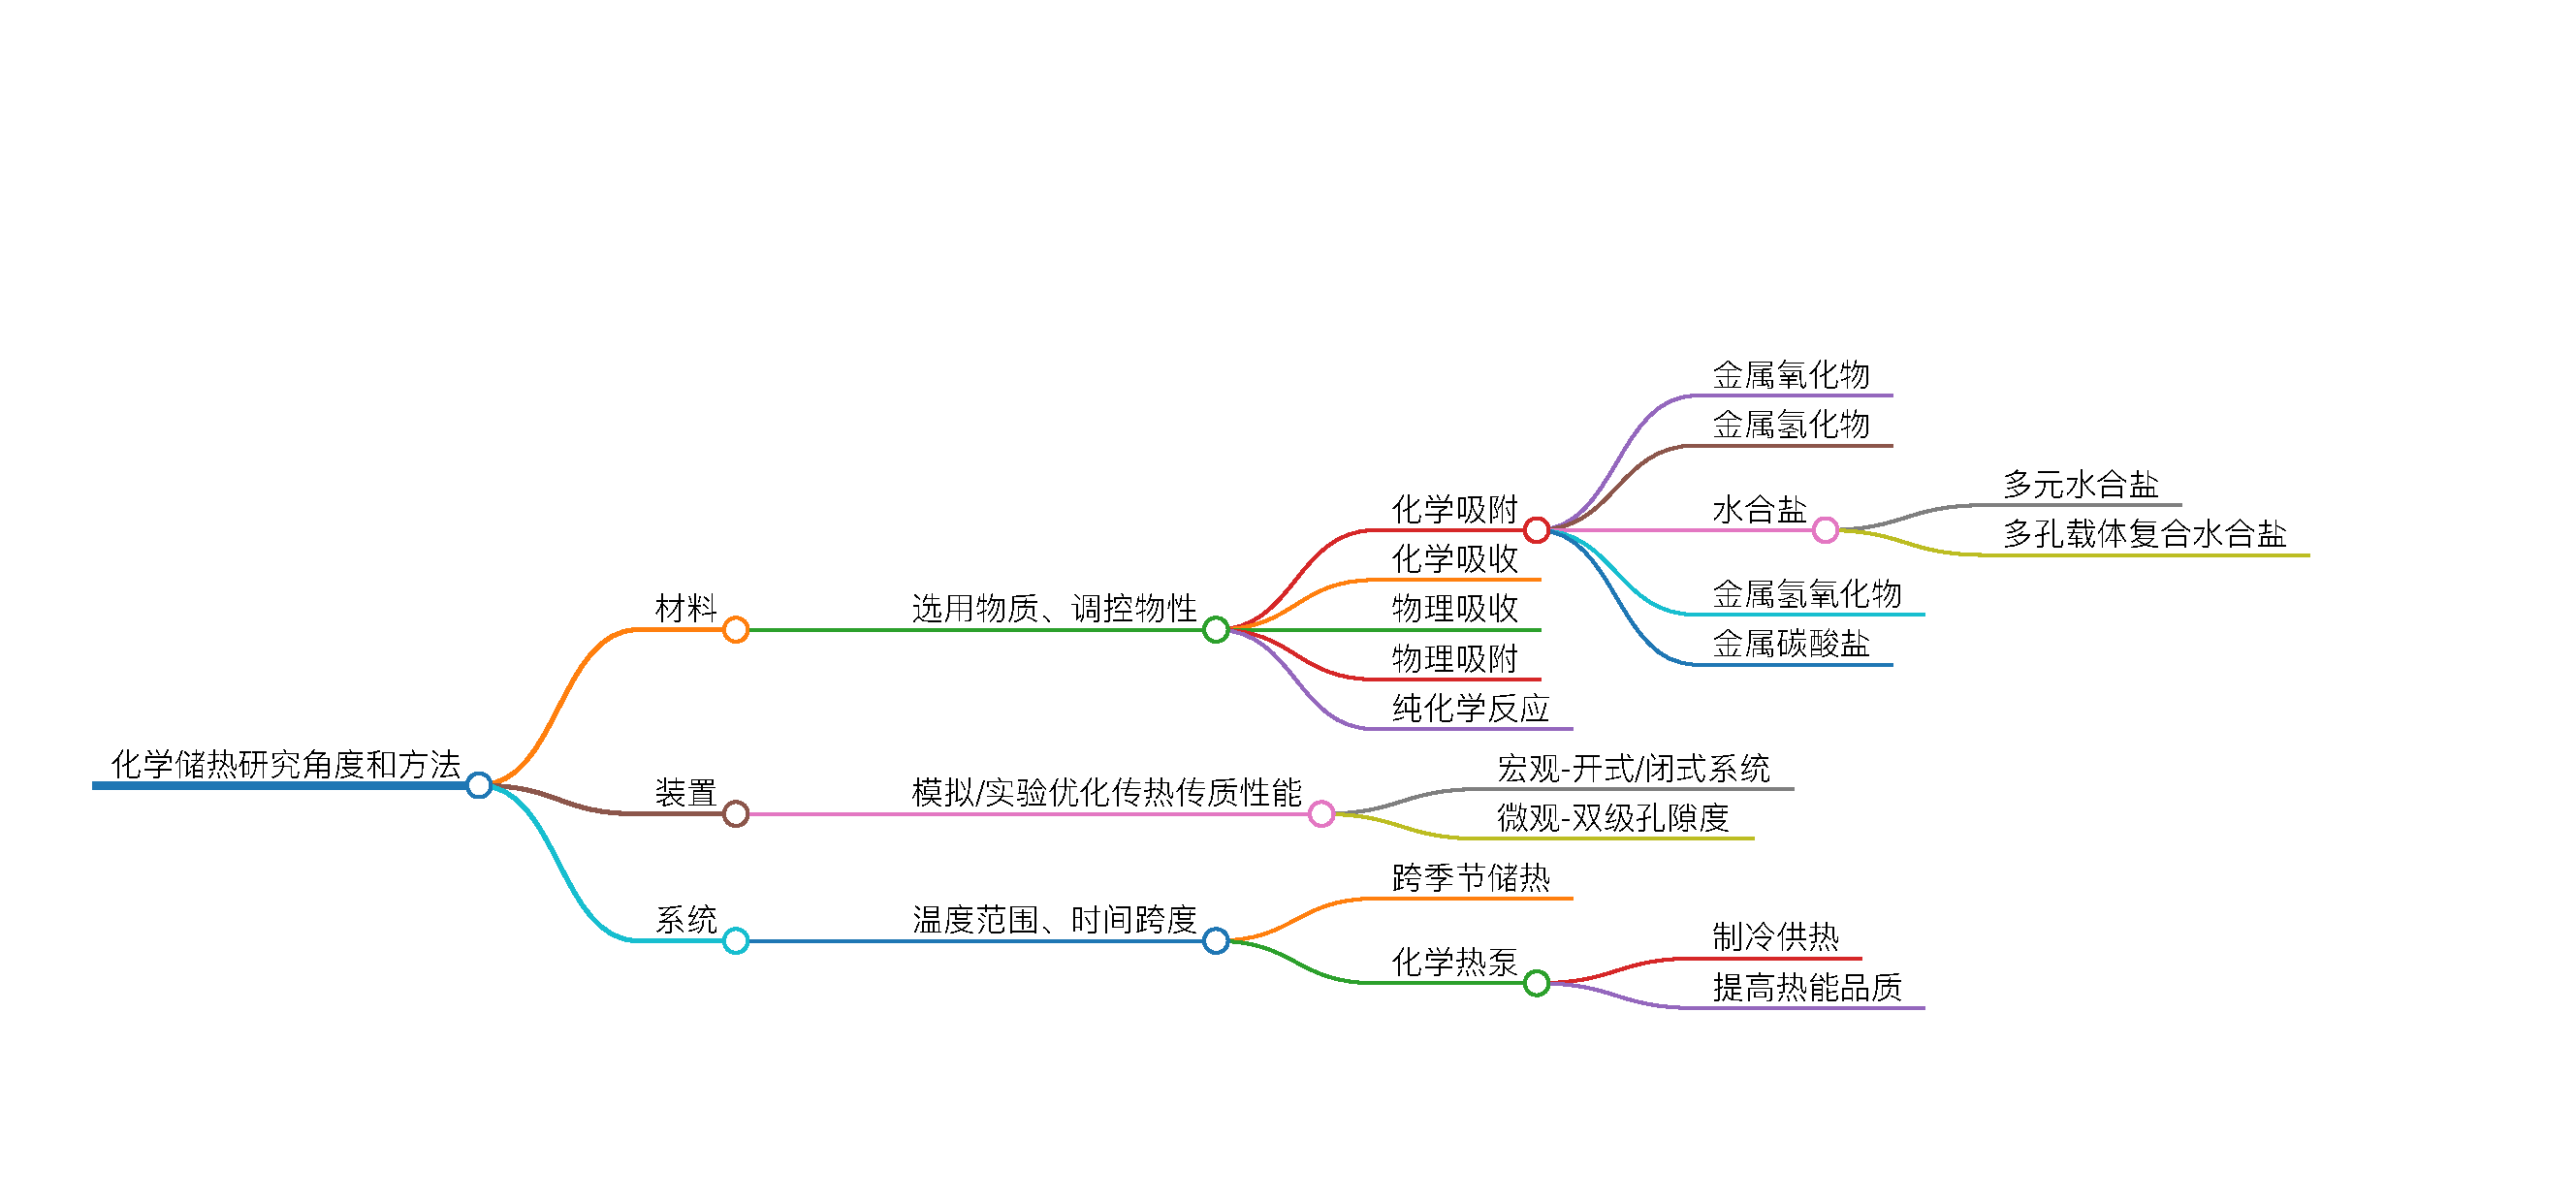
\includegraphics[width=\textwidth]{image/CHS研究角度和方法.pdf}
    \caption{研究角度和方法}
    \label{fig:研究角度}
\end{figure}
\begin{figure}[H]
    \centering
    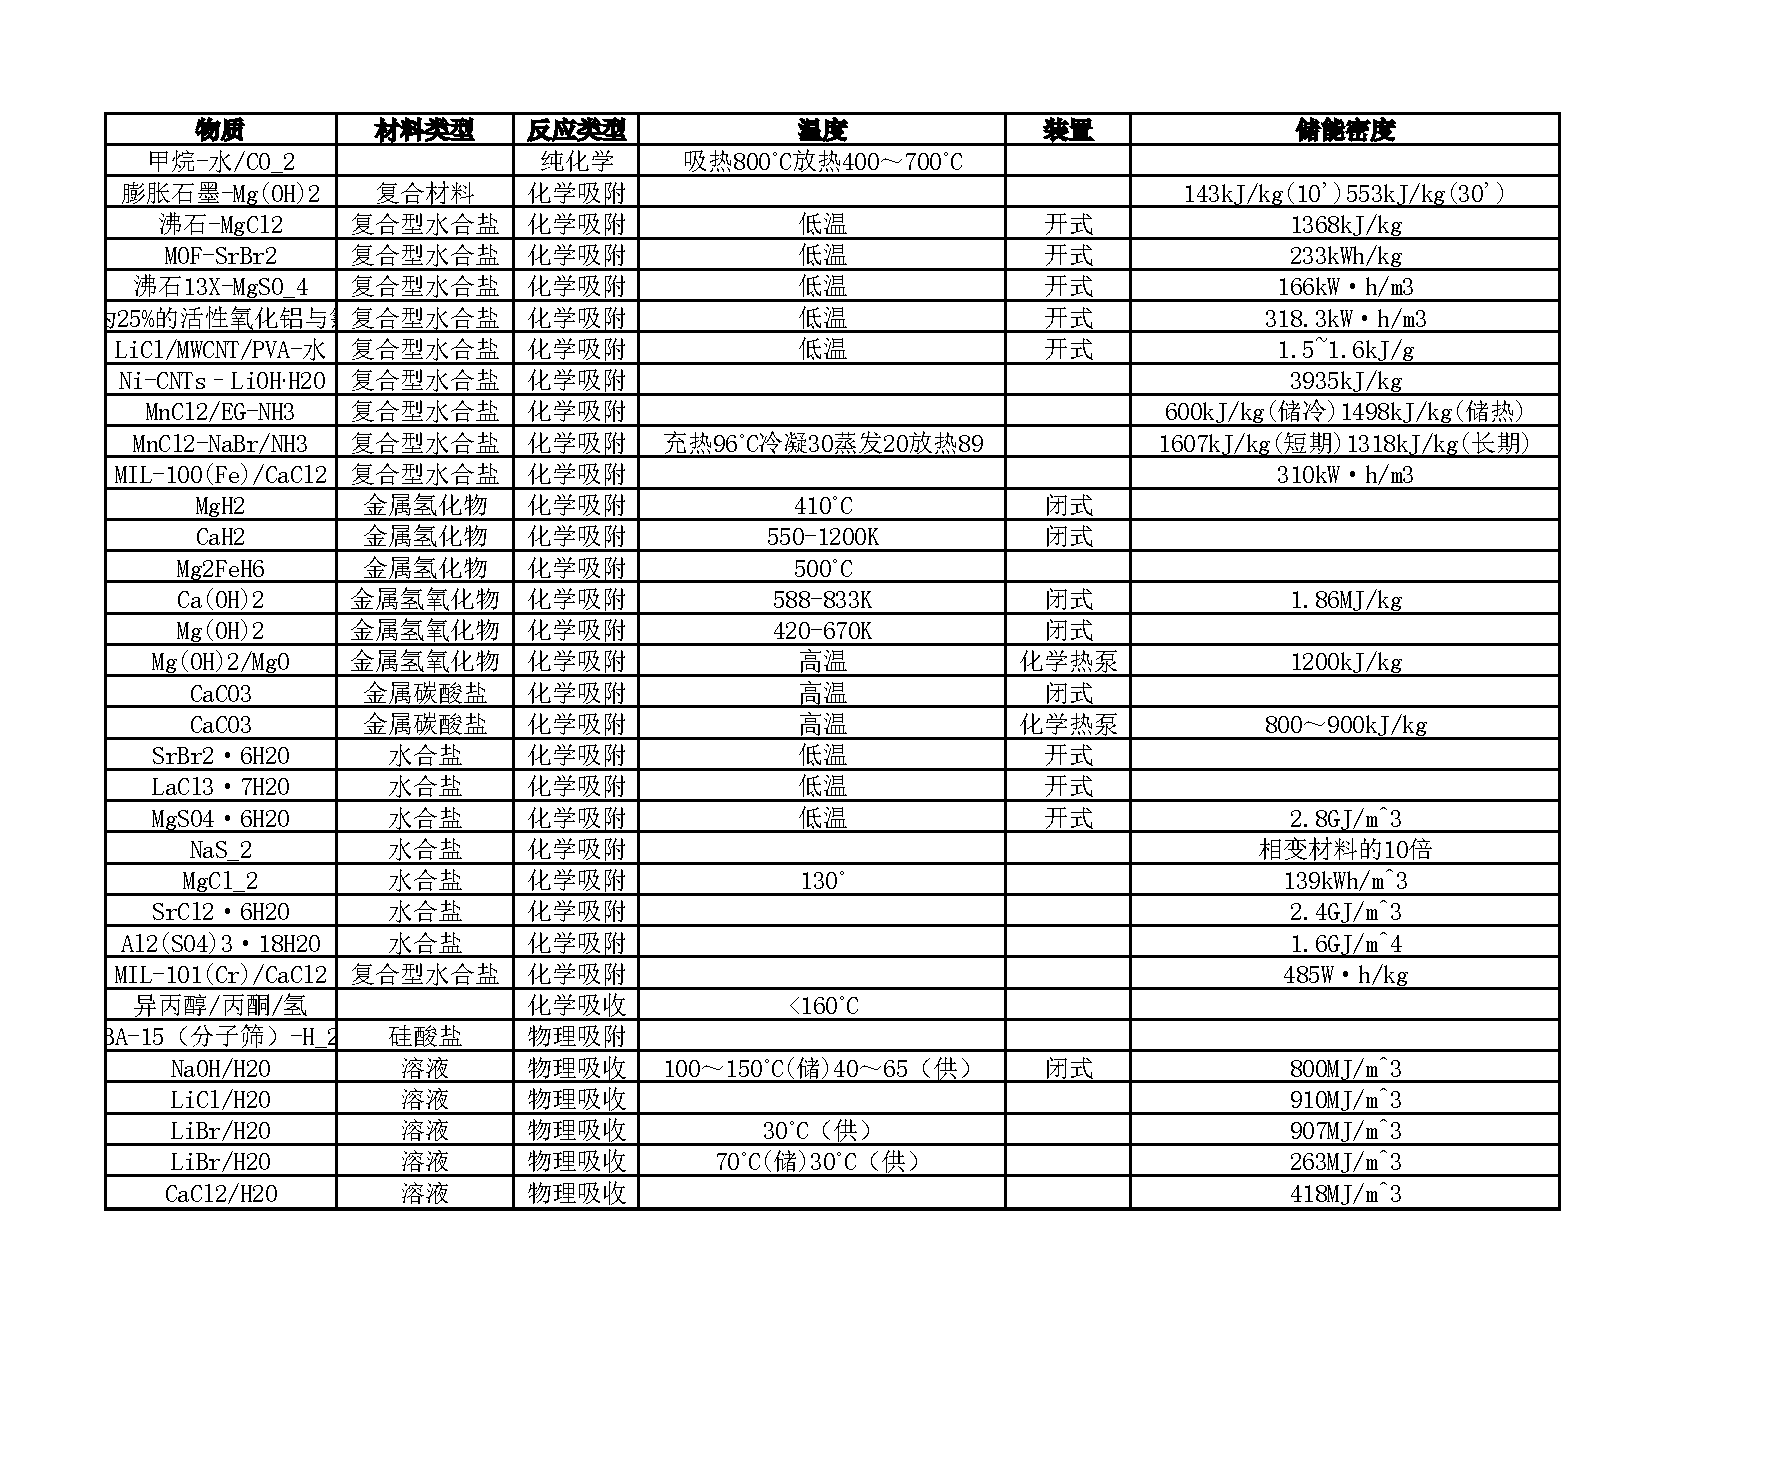
\includegraphics[width=\textwidth]{image/性能比较.pdf}
    \caption{材料及性能比较(草稿)}
    \label{fig:材料对比}
\end{figure}

包含全部论文重点和思维框架的阅读笔记请点击\href{https://github.com/LamGaahou/CHS/blob/main/reports/image/Markmap.pdf}{\color{blue}网页链接}。


\section*{课程学习}

本学期选课20学分,其中专业课包括计算热物理、高等工程热力学、计算流体与传热传质、能源转化中的催化与传质。

本周在计算热物理课程中,我学习了热物理问题的控制方程,偏微分方程的数学、物理分类,有限差分法离散的概念。掌握了拿到某一个偏微分方程后用傅立叶变换法和特征法进行类别判断并与物理问题类别对应的方法;掌握了8种差分算子、基于泰勒展开的差分格式,以及对某特定方程设计迎风格式对方法。

在高等工程热力学课程学习中,我复习了热力学的基本概念、热力学第一、二定律,更深入地学习了热力学第二定律构建可逆过程和孤立系统进行计算的方法,将不可逆过程熵变的计算分成摩擦、温差传热、节流、混合、过冷凝固等多种情况分别分析计算。

在计算流体与传热传质课程中,我学习了是用Gambit-Fluent软件进行数值计算的各种理论知识,包括数值计算的步骤、各种CFD解法,以及各种常用术语。

在能源转化中的催化与传质课程中,我了解了催化材料学的几个简单概念,包括几种分子筛的特性,尤其是钛硅分子筛的结构组成、催化氧化活性机理和择性催化原理。


\end{document}
